\chapter{Background}
\renewcommand{\baselinestretch}{\mystretch}
\label{chap:Back}
%\setlength{\parindent}{0pt}
\PARstart{B}{ack} ground theory, related research and existing tool will be provided in this chapter with detailed illustration. The first section 2.1 will further describe the fuzz testing model selection foundation. The design trade-off was considered between three mainstream model type: black box, grey box and white box. Following section introduce the tested hardware synthesis tool: Berkeley design ABC with its highlights and innovative algorithms. In the final section, the investigation and evaluation of existing fuzz testing tool in hardware synthesis: VlogHammer will be presented.
\section{Fuzz testing and model selection}
As mentioned before, the fuzz testing was pioneered by Dr.Barton Miller. Through 20 years development, it has been matured in software validation and security testing area. Microsoft's Springfield Project applied fuzzing as a service. OSS-Fuzz Continue from Google provide fuzz testing for open-source projects. According to the acknowledge degree of inside structure or code of DUT, the fuzz testing model can be ranked as white-box, grey-box and black-box.
\subsection{Black-box fuzzing}
The Black-box fuzzing is regarded as a random testing method which only considers the correctness of the output results or function. It based on the pre-defined specified or required input, called seeded input \cite{nidhra2012black}. The inside structure and operation principle are not concerned in this kind of test model.Fig \ref{fig:balckbox} shows the construction of the black-box model. 
\begin{figure}[htbp]
    \centering
    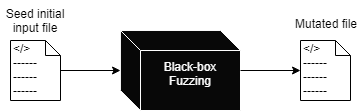
\includegraphics[scale=0.8]{MScThesisTemplate/Figs/balckbox.png}
    \caption{Black-box fuzzing}
    \label{fig:balckbox}
\end{figure}

Mutation is the important characteristic of black box fuzzing. With a valid initial seed, the output of test generator can be randomly mutates to other test-generation heuristics \cite{bounimova2013billions}. The DUT's bugs or vulnerabilities are expected to be evoked by the randomly generalised inputs. Black-box testing is a cost-effective method in bug finding. According to prescription of multinational technology company like Microsoft \cite{bounimova2013billions}, black-box fuzzing is a compulsory procedure of every newly designed device or programmed software. It is knows as "Security Development Lifecycle" \cite{howard2006security} in Microsoft product manual. However, the disadvantage of the black-box fuzzing is relative low code coverage and bug missing. The following short program shows that the probability of triggering the conditional branch \texttt{then} is $1/2^{32}$. Because \texttt{int} type is a 32-bit long parameter and only one corresponding number \texttt{2019} can induce the error issue.

\begin{lstlisting}[float=htb,
        label=lstcode,
        language=C++,
        basicstyle={\ttfamily},
        keywordstyle=\color{blue}, 
        commentstyle=\color{CPPGreen},
        escapeinside=``,
        %breaklines,
       xleftmargin=2em,xrightmargin=2em, aboveskip=1em,
        tabsize=4]
int fuzz(int x){
    int y = x + 1;
    if (y == 2019) 
        abort();//Bug location
    return 0;
}
\end{lstlisting}

\subsubsection{Csmith}
Csmith is a typical implementation of blaxk-box fuzzing. As Xuejun Yang, Yang Chen et al, mentioned in their paper \cite{Yang:2011:FUB:1993316.1993532} they designed Csmith as a "randomised test-case generation tool". The generated C program by Csmith involved most kinds of C expressions and statements defined in C99 standard. Other commonly used features in C language such as control flow (\texttt{if/else},\texttt{for} loop, \texttt{break}), variable definition (\texttt{int},\texttt{char}), operation (arithmetic, logical and bitwise) are also covered in Csmith. The structure of the Csmith shows in the Fig. \ref{Fig:csmith}. The test harness has been passed to three different compilers to execute it. Comparison among the three compilers, the minority result indicates that it has large probability containing bugs or vulnerabilities. 

Avoid inadequacies for the compilers, each generated program by Csmith has a unique interpretation. Csmith's C program generation follows top-down architecture. The global environment of Csmith describe the highest level definitions. The local environment defines three information: current call chain, objects and all in-scope pointers \cite{Yang:2011:FUB:1993316.1993532}. Guided by probability table, the Csmith construct the c code file step by step from basic \texttt{main} to branch function and sub-objects. The researchers spent three years to find serves, previous unknown bugs in mainstream C compilers such as GCC, LLVM and other commercial tools. End till the publish of their paper, the number of detected unknown bugs is 325 and has been reported to the compiler developer. These bugs and vulnerabilities including compiler crash and return wrong compiling output results \cite{klees2018evaluating}. The quantitative analysis of Csmith shows that the code coverage of Csmith is high in line(75.58\%) and function(82.41\%), but low in branch(46.26\%). The cumulative distinct crash error of Csmith is 86 which in significantly.

Csmith proves that black-box fuzzing is a worth considering model in hardware synthesis tool testing. Because the impressive effectiveness of bug finding, detected 325 unknown bugs in short 3 years. The design structure is easy to understand and implement.

\begin{figure}[htbp]
\centering
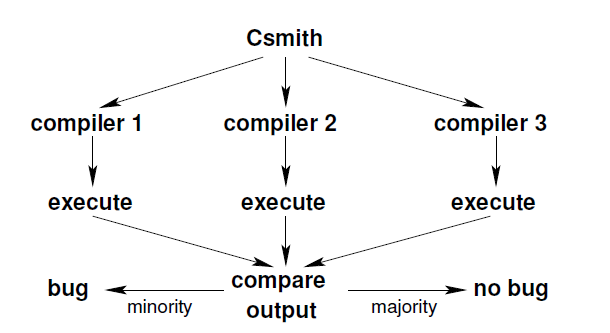
\includegraphics[scale=0.6]{MScThesisTemplate/Figs/Csmith.PNG}
\caption{Csmith architecture \cite{Yang:2011:FUB:1993316.1993532}}
\label{Fig:csmith}
\end{figure}

\subsection{White-box fuzzing}
White-box fuzzing is an alternative fuzz testing method. With the development of systematic dynamic test generation \cite{godefroid2005dart}, the white-box fuzzing has been extended from unit-level to integration and system level. The white-box fuzzer will dynamically operate the symbolic executed input until all feasible path of the DUT has been swept through. Testing structure of the white-box fuzzing shapes a "Tree" which is provided in Fig.\ref{fig:whitebox}. Using above program in \ref{lstcode} as example, the initial seed value of input \texttt{x} is \texttt{1} and \texttt{y = x + 1} which will assign \texttt{2} to \texttt{y}. The path constrain \texttt{2} $\neq$ \texttt{2019} yields the execution of conditional branch \texttt{else}. Finishing execution of one conditional branch under such constraint, the next generated input would be \texttt{x = 2018} to allow the execution of the other conditional branch. The input format or other specification do not need to know. Moreover, each individual path of the DUT and internal perspective of the DUT will be egoistic tested. This guarantee the high code coverage of white-box fuzzing. \cite{functest}

Comparing to black-box fuzzing, white-box fuzzing has advantage in full path thorough testing. The testing processes are traceable and easy to automate. In practice, the large scale of execution path of DUT can not be available to be tested. The large number of path can not be precisely within a reasonable time. Besides, white-box fuzzing increase the complexity to testing and reduce the universality. Therefore, the white-box fuzzer might be closely connected with the specific implementation of the DUT. Rewriting the output generated by designed fuzzer may lead assumption failure or occur unnecessary error \cite{nidhra2012black}\cite{bounimova2013billions}. Moreover, white-box fuzzing cost too much computational resource in dynamic symbolic execution. 
\begin{figure}[htb]
    \centering
    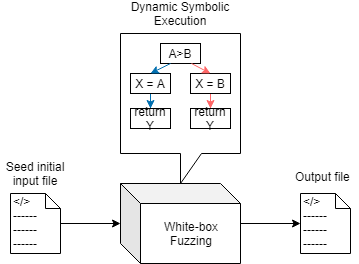
\includegraphics[scale=0.8]{MScThesisTemplate/Figs/whitebox.png}
    \caption{White-box fuzzing}
    \label{fig:whitebox}
\end{figure}
\subsubsection{SAGE}
In the published paper by Ella Bounimova, Patrice Godefroid and David Molnar \cite{bounimova2013billions}, they proposed an constraint-based white-box fuzzer SAGE. The developers aim to generate large numbers of instruction and statements in single symbolic execution. Thus, the generational search strategy of the SAGE was creative and innovative. The first step of symbolic execution will create a path constraint. As they described in their paper \cite{bounimova2013billions}, the rest of the constraints in this path will be solved by a constrain solver and ''placed in a conjunction with the prefix of the path constraint leading to it''. The static result shows that single execution can generate 25,598 full path constraints.

The structure of shows in Fig \ref{Fig:sage}. An initial input would be passed to SAGE to run the program test. If the program crashes, it means that this initial input may trigger a bug. If not, the SAGE will symbolically execute the program with that input and generate the required path constraints. When all the contraint in that path have been solved by the constraints solver, the satisfied constraints would be mapped into \texttt{N} different input to improve the instruction coverage. \texttt{N} constrains would be ranked in terms of the ability of discovering new instructions. The next symbolic execution of SAGE will adopt the highest mark input as its input \cite{bounimova2013billions}.

The result of SAGE show that the SAGE fuzzer can find around 50 unique bugs in 23 days of running it on 200 programs. Comparing with the bug hunting ability of black-box model(352 bugs in three year's testing), the efficiency have been greatly improved. It proves the advantage of white-box in high code coverage and full path through testing. However, the implementation of SAGE used the dynamic systematic generation execution. The structure diagram of SAGE (Fig \ref{Fig:sage}) is much more complicated than the black-box Csmith(Fig \ref{Fig:csmith}). 
\begin{figure}[htb]
\centering
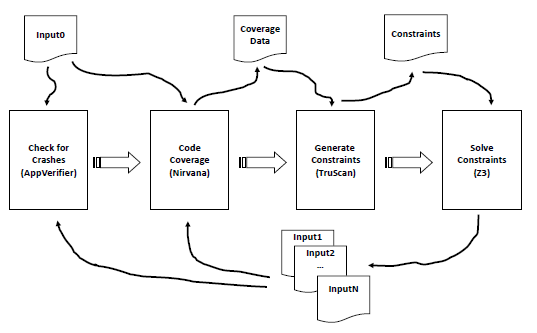
\includegraphics[scale=0.8]{MScThesisTemplate/Figs/sage.PNG}
\caption{SAGE architecture\cite{bounimova2013billions}}
\label{Fig:sage}
\end{figure}

\subsection{Tradeoff: Grey-box fuzzing}
Leveraging the pros and cons of black-box fuzzing and white-box fuzzing, this project decided to use the intermediate model: grey-box fuzzing model. Grey-box fuzzing integrate the features of black-box and white-box. It partly know the inside structure, code and algorithm of DUT but the test aim is correctness of output results based. It is beneficial in the hardware synthesis tool testing. Because the input file of a hardware synthesis tool require a specific format and the input HDL file should be synthesizable. For example, if the generated HDL file is a test-bench, it indeed a valid input file of the hardware synthesis tool but the synthesis tool can not yield a synthesised netlist. In addition, the output netlist circuit of the DUT not only expected to correctly execution but also expected to be synthesised in a optimised way. For instance, the \cite{havrikov2017efficient} %Need an example.
In addition,  
The detail part of this projects fuzzer will be presented in the methodology section of chapter 3.

\section{Hardware synthesis: Berkeley designed ABC}
ABC is a powerful synthesis and formal verification tool in hardware designs. It was developed by Robert Brayton and Alan Mishchenko in University of California, Berkeley. Since 2005, ABC has been gaining momentum and attention to be a ''public-domain'' tool in hardware logical synthesis and verification \cite{ABC}. In this project, ABC was used as a synthesis tool. As a result, the verification function of ABC was neglected. 
\subsection{Selection motivation}
The first reasons of selecting ABC as a DUT is that ABC occupies a dominant position in academic research. The user of ABC are University of Colorado (Boulder), Cornell University and University of California (Berkeley). If a bug or Vulnerability was found in the ABC, it is beneficial for the academic staff to avoid wrong scientific research. 

Secondly, the open-source feature of ABC is a huge merit. As a open-source tool of Electronic Design Automation(EDA), ABC is source code can be forked from Github \url{https://github.com/berkeley-abc/abc}. The open source mode can improve the software's reliability due to the contribution of thousands of independent programmers in software testing and bugs fixing.\cite{laurent2004understanding} With the source code of the ABC, the design of the fuzz testing software could use the grey-box fuzzing model. As discussed in above section, no doubt that the programmed testing tool will be more efficient and pertinence. Besides, the access of viewing and modifying source code of ABC allow us to inject bugs to ABC in future analysis.

The third reason of select ABC is its high efficiency. The synthesis method of ABC has switched from multi-level valued to binary And-Inverter Graphs (AIGs). Comparing to its predecessor SIS (developed by research group of UC Berkeley in 1987-1991\cite{ABC}), it saves the runtime and memory space. The scalability of ABC has increased due to the saving in above two aspects.

In addition, ABC attached equivalence checker provided a efficient way in final comparison stage of this project. The equivalence checker of ABC can handle both combinatioal and sequential circuit based on SAT sweeping \cite{satsweep,kuehlmann2001circuit}. Two circuits will be transformed into an equivalence checking miter which is consisted of EXOR gates and OR gates. 
The inputs of the original circuit will be transmitted to EXOR gates and ORed to yield a output of the miter. This equivalence checker has been awarded to out of three categories at hardware model checking competition at CAV 2008. It certified that the checking result of the equivalence is reliable.

\subsection{Highlights and commands}%这一部分还需要大改
Hardware synthesis tool is expected to convert a high-level HDL into an optimised gate-level representation (Netlist). The transformation need to satisfy some criteria such as optimise the gate number, logic level and node number. ABC combines scalable logic optimization based on AIG , optimal-delay DAG-based technology mapping for look-up tables and standard cells, and innovative algorithms for sequential synthesis and verification \cite{ABC}.\\
\textbf{Multiple in-out parse:}\\
\textbf{And-Inverter Graphs:}


The following tabale shows some circuit optimisation instruction involved in this project.
\begin{table}[!htbp]
    \centering
    \begin{tabular}{c|c|m{8cm}}
        \hline
       Command type & Command name & Function\\
        \hline
     \multirow{3}{*}{Synthesis}&\textbf{\texttt{balance}} & Assumes that the input is an AIG and creates an equivalent AIG having the minimum delay, measured using logic levels of two-input AND-gates. The inverters do not count towards the number of logic levels. The resulting AIG is derived by algebraic balancing of the multi-input AND-gates contained in the original AIG. The balancing is applied in the topological order and selects the minimum delay tree-decomposition of each multi-input AND-gate. Balancing takes into account the arrival times of primary inputs, which can be represented in BLIF.\\
     \cline{2-3}
     & \textbf{\texttt{strash}}&Transforms the current network into an AIG by one-level structural hashing. The resulting AIG is a logic network composed of two-input AND gates and inverters represented as complemented attributes on the edges. Structural hashing is a purely combinational transformation, which does not modify the number and positions of latches.\\
     \cline{2-3}
     & \textbf{\texttt{cycle}}&Simulates the sequential network with random input and updates its current state.\\
     \hline
     \multirow{2}{*}{Read}&\textbf{\texttt{read\_verilog}}&Parses the input file in a very limited subset of structural Verilog, which includes all the keywords and directives needed for reading IWLS 2002 Benchmarks and  IWLS 2005 Benchmarks. Before reading the latter, make sure the Cadence library is loaded into ABC using command \texttt{read\_library cadence.genlib}. When the library is loaded, use command \texttt{r –m <file.v>}\\
     \cline{2-3}
     & \textbf{\texttt{read\_aiger}} & Reads the combinational AIG in binary AIGER format developed by Armin Biere. This format is very compact and leads to a substantial reduction in the reading/writing times.\\
     \hline
     \multirow{2}{*}{Write}&\textbf{\texttt{write\_verilog}}& Outputs the network using technology-independent Verilog.\\
     \cline{2-3}
     & \textbf{\texttt{write\_verilog}}& Outputs the network using technology-independent Verilog.\\
     \hline
     
\end{tabular}

    \caption{Main commands related in this project\cite{manual2006quick}}
    \label{tab:my_label}
\end{table}



\section{Existing bug-hunting tool in hardware synthesis}
VlogHammer is a current existing regression Verilog test software to verify the circuit correctness of the Verilog \cite{wolf2016yosys}. As a powerful fuzzer VlogHammer can generate different types of combinational logic circuit in Verilog. The algorithm used by VlogHammer is based on divide-and-conquer.

\section{Related work}